\documentclass{article}
\usepackage[utf8]{inputenc}

\usepackage{float}
\usepackage{natbib}
\usepackage{graphicx}
\usepackage[export]{adjustbox}
\usepackage{multirow}
\usepackage{hyperref}
\usepackage{titlesec}
\usepackage{ragged2e}


\documentclass{article}
\usepackage{bera}% optional: just to have a nice mono-spaced font
\usepackage{listings}
\usepackage{xcolor}

\colorlet{punct}{red!60!black}
\definecolor{background}{HTML}{EEEEEE}
\definecolor{delim}{RGB}{20,105,176}
\colorlet{numb}{magenta!60!black}

\lstdefinelanguage{json}{
    basicstyle=\normalfont\ttfamily,
    numbers=left,
    numberstyle=\scriptsize,
    stepnumber=1,
    numbersep=8pt,
    showstringspaces=false,
    breaklines=true,
    frame=lines,
    backgroundcolor=\color{background},
    literate=
     *{0}{{{\color{numb}0}}}{1}
      {1}{{{\color{numb}1}}}{1}
      {2}{{{\color{numb}2}}}{1}
      {3}{{{\color{numb}3}}}{1}
      {4}{{{\color{numb}4}}}{1}
      {5}{{{\color{numb}5}}}{1}
      {6}{{{\color{numb}6}}}{1}
      {7}{{{\color{numb}7}}}{1}
      {8}{{{\color{numb}8}}}{1}
      {9}{{{\color{numb}9}}}{1}
      {:}{{{\color{punct}{:}}}}{1}
      {,}{{{\color{punct}{,}}}}{1}
      {\{}{{{\color{delim}{\{}}}}{1}
      {\}}{{{\color{delim}{\}}}}}{1}
      {[}{{{\color{delim}{[}}}}{1}
      {]}{{{\color{delim}{]}}}}{1},
}




\begin{document}
\title{COS301 Team Gamma: UserManagementAPI Team Goals}
\begin{figure}
    \centering
    
\includegraphics[width=\textwidth]{logo.png}
\end{figure}
\date{March 2020}

\maketitle

\section{Introduction}
This document describes the responsibilities and all deliverables for the \\UserManagementAPI Team.
\\ \\
Demo \#1 Due Date: Thursday 12 March 20:00
\newpage

\section{Organisation}
\subsection{ClickUP}
You need to elect a team leader if you have not done so already. Work together with this member to create tasks and sub-tasks for each member in your team on \url{http://clickup.com} (on the COS301 workspace you have been invited to). \\

\begin{figure}[h]
    \centering
    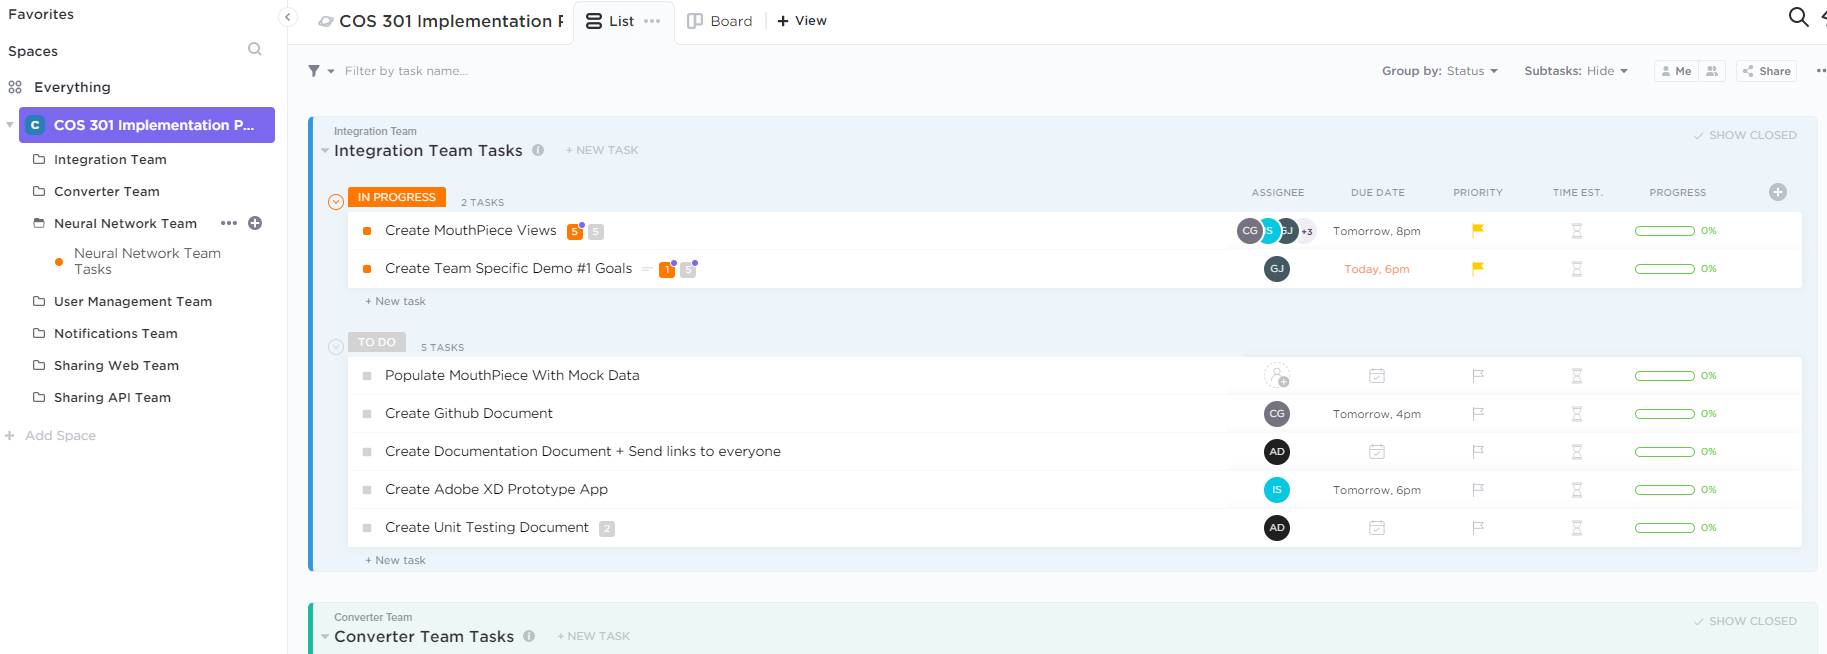
\includegraphics[width=\textwidth]{clickup.png}
\end{figure}

Ensure that you indicate progress and mark tasks as complete. This page will be displayed at the demo.

\subsection{Slack}
Although we have created a WhatsApp group - we do still find it easier for in-group discussions to happen on the slack channels. Simply login to \url{http://cos-301.slack.com}

\newpage

\section{Overall Team Tasks}
These are the tasks to be done by your team for the final product (not specifically Friday's demo).

\begin{itemize}
    \item Design and implement a database to store all information pertaining to User Profiles \& Preferences (MySQL)
    \item Implement a REST API that will
    \begin{itemize}
        \item Create user profiles
        \item Update user profiles
        \item Delete user profiles
        \item Query user profiles
        \item Authenticate users (merely respond with JSON to say whether the login is valid or not)
        \item All requests and responses to be done in JSON, as POST requests
        \item Take special care with security in PHP (encrypt data)
    \end{itemize}
    \item The API will be stored and ran at: \url{http://teamgamma.ga/api/usermanagementapi.php}
\end{itemize}

\vspace{1cm}

\begin{center}
   \textit{The tasks are always subject to change, but we have tried our utmost best to sketch out the entire project ahead.}
\end{center}

\newpage


\section{Team Tasks for Friday}

\subsection{Documentation}
\textbf{All documentation to be created in Overleaf}

\subsubsection{Database Design}
You are required to document the Database tables and attributes with relationships. Write descriptions for each table and attribute. Create a complete ERD diagram and add it to the document. This should be as close to the final product as possible.

\begin{figure}[h]
    \centering
    \includegraphics[width=\textwidth]{erd.png}
    \caption{Example ERD diagram}
\end{figure}

\newpage

\subsubsection{API Interface}
You are required to document the entire API interface. This includes listing all the HTTP requests the API will serve (e.g. authenticateUser). \textbf{Some requests will inevitably change in the future, so rather get down to implementing it for Friday than overthinking it}\\

\textbf{More specifically:}
\begin{itemize}
    \item Create every HTTP request as a heading in the document
    \item Provide a description as to the functionality of the request
    \item Provide a sample JSON request (to be sent to server) alongside a sample JSON response (to be sent back to client)
\end{itemize}

\textbf{Example JSON Request:}
\begin{lstlisting}
{
   "requestType" : "authenticateUser",
   "username" : "giovanni",
   "password" : "some encrypted data"
   "responseOptions" : 
   {
   "something" : 5
   "whatever" : true
   }
}
\end{lstlisting}

\begin{center}
   \textit{Please think about the JSON critically - don't merely follow the above example}
\end{center}

\newpage
\subsection{Hosting Environment}
Your team will already deploy your demo for Friday on the Apache web server. You will demo your FTP setup and showcase the live URL.\\

\textbf{Use the following FTP details for the /api/ directory:} 

\begin{itemize}
\begin{itemize}
\item Host: ftp.teamgamma.ga
\item Username: apiteams@teamgamma.ga
\item Password: zVrikkNBJa3
\item Port: 21
\end{itemize}
\end{itemize}

Your FTP login details are rooted in: \url{http://teamgamma.ga/api/}. i.e. any uploads will be visible on that URL. Create your API as \textbf{usermanagementapi.php} (it's already in the directory). This is the same url that will be used for deployment.

\begin{center}
   \textit{Ensure that you don't overwrite any of the other API team's files.}
\end{center}

\textbf{Use the following Database details:} 

\begin{itemize}
    \begin{itemize}
        \item Host: teamgamma.ga
        \item Database name: teamgamma\_usermanagementapi
        \item Username: teamgamma\_usermanagement
        \item Password: xZE1UlkYA4
    \end{itemize}
\end{itemize}

\begin{center}
   \textit{If you have any issues with the hosting (permission issues etc), or require additional server resources, contact Giovanni (on Slack).}
\end{center}

\newpage

\subsection{Implementation}
\subsubsection{Database}
You are required to implement your ERD diagram as a live MySQL Database (details above).  \\

\textbf{Create:}
\begin{itemize}
    \item All the tables
    \item All the attributes and relationships
    \item Fill in some mock data (at least two entries in each table where applicable)
\end{itemize}

Demo the database via the terminal on one of your member's laptops. (i.e. log in to database, list tables, list data etc)

\subsubsection{PHP Api}
You are required to implement at least three working HTTP requests on the apache server \url(http://teamgamma/api/usermanagementapi.php) (details above).  \\
\textbf{In other words:}
\begin{itemize}
    \item Establish the connection from PHP to the Database (don't worry about Singletons etc. for now, we can implement those later)
    \item Write 3 working HTTP requests 
    \item Ensure you are accepting requests as JSON, POST requests only.
    \item Query the database and send back the result as a JSON formatted response
\end{itemize}
\\

Demo the API via \url{https://www.postman.com/}


\subsubsection{Unit Testing}
Describe how your team will implement unit testing. Better yet - implement it in the Demo where possible.


\end{document}